% Week 5: the research question and the prior beliefs behind it. Numbers and citations are carried
% over from thesis/risk_models/01_model_features_v2.tex and thesis/week4/locked_tortuosity_metrics.tex.
% Nothing new was read for this note.
\documentclass[11pt,a4paper]{article}
\usepackage[margin=1in]{geometry}
\usepackage{amsmath}
\usepackage{microtype}
\usepackage{graphicx}
\usepackage{float}
\graphicspath{{../../figures/}}
\usepackage[backend=biber,style=numeric,sorting=none]{biblatex}
\addbibresource{../refs.bib}
\DeclareSourcemap{\maps[datatype=bibtex]{\map{\step[fieldset=note,null]}\map{\step[fieldset=abstract,null]}}}
\usepackage[colorlinks=true,linkcolor=blue,citecolor=blue,urlcolor=blue]{hyperref}

\title{Week 5: the research question}
\author{}
\date{}

\begin{document}
\maketitle


\section{Can the geometry of a healthy coronary tree tell us who will develop plaque?}

\noindent Plaque is the build-up of cholesterol, inflammatory cells and fibrous tissue inside the
artery wall, which narrows the vessel and can rupture to cause a heart attack.
Every segment of the coronary tree is exposed to the same systemic risk factors, such as high blood
pressure, high cholesterol and smoking.
Yet plaque forms at specific sites rather than uniformly along the vessels
\cite{chatzizisis2007ess}.
If the cause were only in the blood, plaque would be spread evenly, so something local at those sites
must add to the risk.

\begin{figure}[H]
  \centering
  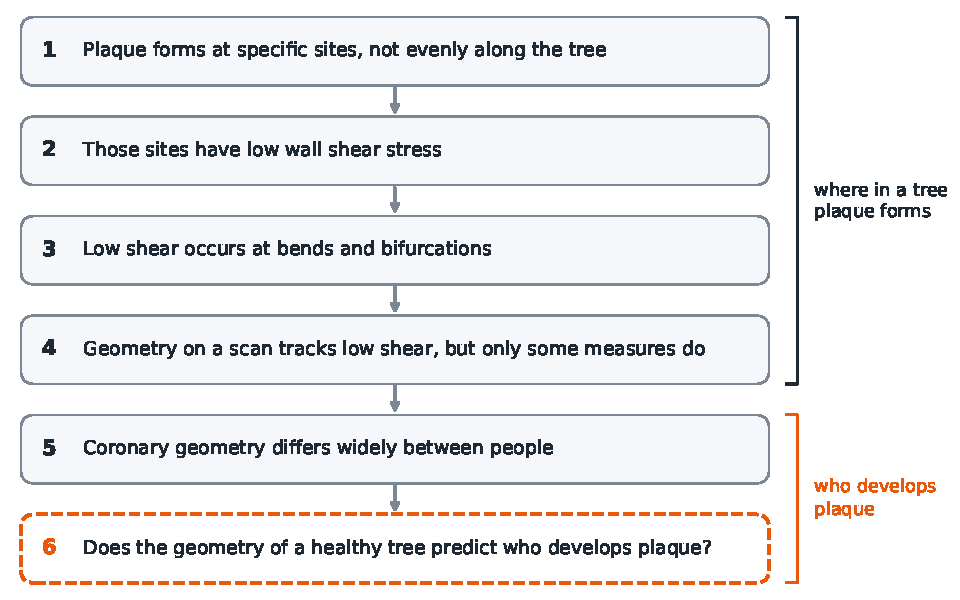
\includegraphics[width=0.9\textwidth]{rq_chain.pdf}
  \caption{The reasoning behind the research question.
    Steps 1 to 4 concern where in a single coronary tree plaque forms, and each rests on published
    work.
    Step 5 is also documented, but step 6, whether the shape of a healthy tree predicts who develops
    plaque, has not been tested.}
  \label{fig:rq-chain}
\end{figure}

\medskip
\noindent \textbf{The local factor is low wall shear stress}

\noindent Blood flowing along an artery drags on the wall it passes, and that frictional drag is the
wall shear stress (WSS).
For steady flow at flow rate $Q$ through a tube of radius $R$, it scales as $Q/R^{3}$, so the drag
changes wherever the vessel widens, narrows, bends or divides \cite{rampidis2022geometry}.
The endothelium, the single layer of cells lining the artery, senses this drag.
Where it is high and steady the cells stay quiescent; where it is low, or reverses direction over
the cardiac cycle, they turn inflamed and let cholesterol into the wall, and it is there that plaque
starts and grows \cite{chatzizisis2007ess}.

\begin{figure}[H]
  \centering
  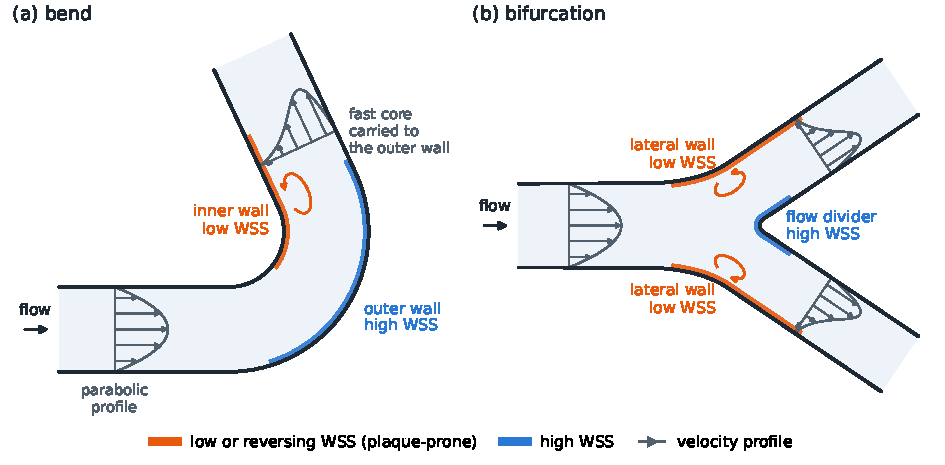
\includegraphics[width=\textwidth]{wss_schematic.pdf}
  \caption{The shape of a vessel decides where its wall feels low shear.
    (a) In a bend, the fast core of the flow is carried to the outer wall, which feels high wall
    shear stress (WSS), while flow along the inner wall slows and can recirculate.
    (b) At a bifurcation, the fastest flow enters each branch next to the flow divider, which feels
    high WSS, while flow along the lateral walls separates and recirculates.
    The orange walls are where Asakura and Karino found almost all plaque in five coronary trees
    \cite{asakura1990flow}.
    Schematic; the velocity profiles are drawn by hand, not simulated.}
  \label{fig:rq-wss}
\end{figure}

\medskip
\noindent \textbf{Low shear occurs at geometrically distinctive sites}

\noindent Tracing the flow through five human coronary trees after death, Asakura and Karino found
almost every plaque at one of two kinds of site: the outer walls of the daughter branches at
bifurcations and the inner walls of bends, both where the flow slowed or recirculated
\cite{asakura1990flow} (Figure~\ref{fig:rq-wss}).
At a bifurcation, where one vessel divides into two, the fast flow enters each branch next to the
flow divider, while flow along the outer walls of the branches separates and recirculates.
In a bend, the fast core of the flow is carried to the outer wall by its own momentum, leaving slow
flow along the inner wall.
Plaque also concentrates in the proximal segments near the origin of each artery, where the major
bifurcations cluster.


\medskip
\noindent \textbf{Low shear can be estimated from vessel geometry}

\noindent Knowing that bends and bifurcations carry low shear does not say how to measure them:
low-shear sites are normally found with a flow simulation, which is slow, needs specialist setup and
depends on assumed flow conditions \cite{griffo2026wss,shen2026geometry}.
Recent studies show that the geometry of the vessel alone tracks the shear, but only if it is
measured the right way.
In 127 patients without coronary artery disease, Kashyap et al.\ found average curvature to be the
measure most closely tied to low shear, whereas the tortuosity index, the ratio of a vessel's length
to the straight-line distance between its ends and the measure most used in the literature, showed
no correlation ($p = 0.86$) \cite{kashyap2022tortuosity} (Figure~\ref{fig:rq-curvature}).
A neural network trained on 1078 vessel segments from 748 patients estimated the pattern of shear
along a vessel from its shape alone, agreeing with the full simulation at $R = 0.89$, although these
vessels were reconstructed from invasive angiography rather than CT \cite{griffo2026wss}.
Geometry therefore carries information about where shear is low, but which measure is used
matters.

\begin{figure}[H]
  \centering
  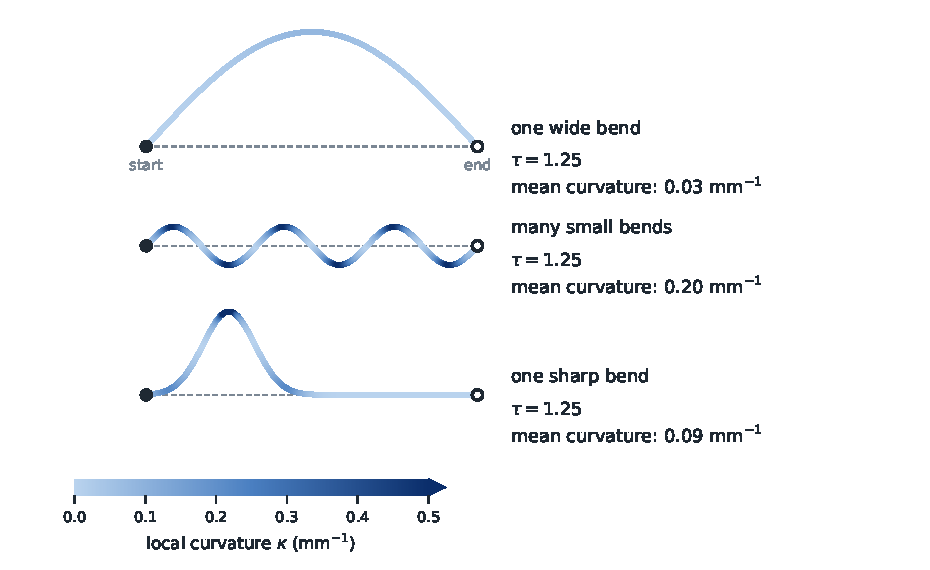
\includegraphics[width=0.85\textwidth]{rq_curvature.pdf}
  \caption{The tortuosity index cannot tell these three vessels apart, but curvature can.
    Each synthetic centerline is 50\,mm long between ends 40\,mm apart, so all three share the
    tortuosity index $\tau = 1.25$, yet their mean curvature differs sixfold.
    Color shows local curvature $\kappa$, the inverse of the radius of the bend at each point.
    Curvature, not $\tau$, tracked low shear in 127 patients \cite{kashyap2022tortuosity}.}
  \label{fig:rq-curvature}
\end{figure}

\medskip
\noindent \textbf{From where plaque forms to who develops it}

\noindent The steps so far say where in a given tree plaque is likely to form: plaque forms where
shear is low, shear is low at bends and bifurcations, and these can be measured from the shape of
the tree (Figure~\ref{fig:rq-chain}).
The next step is from sites to people.
Coronary geometry differs widely between individuals: in 196 patients examined with coronary CT
angiography (CCTA), the angle between the left anterior descending (LAD) and left circumflex
(LCX) arteries ranged from $35.5^\circ$ to $178^\circ$ \cite{temov2016bifurcation} (Figure~\ref{fig:rq-angle}).
Since wall shear stress varies with the geometry, people may differ in geometric properties that indicate their risk of plaque before any disease is present, and these properties can be measured from a CCTA scan.
Showing that one geometric property carries more risk than another requires many people, scanned
while healthy and followed forward in time to see who develops plaque.

\begin{figure}[H]
  \centering
  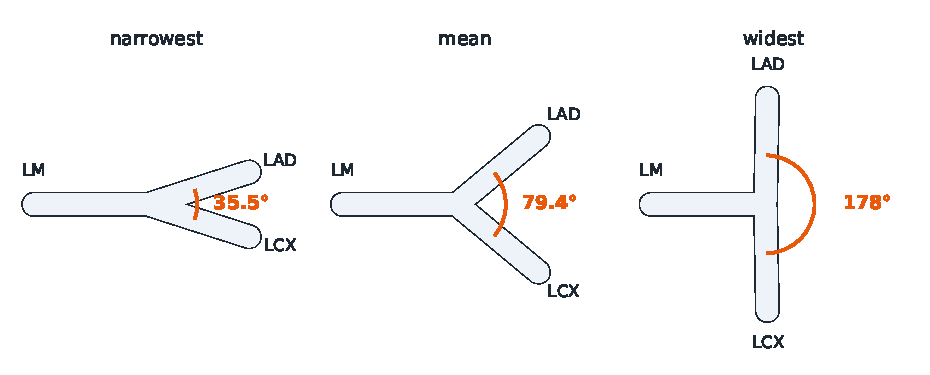
\includegraphics[width=0.85\textwidth]{rq_angle.pdf}
  \caption{The same bifurcation takes very different shapes in different people.
    Where the left main (LM) coronary artery divides into the LAD and LCX, the angle between the two
    branches ranged from $35.5^\circ$ to $178^\circ$, with a mean of $79.4^\circ$, in 196 patients
    examined with CCTA \cite{temov2016bifurcation}.
    Schematic, drawn to these three angles.}
  \label{fig:rq-angle}
\end{figure}

\medskip
\noindent \textbf{Predicting future plaque from a healthy tree has not been tested}

\noindent Studies of this kind are essentially missing.
Studies comparing geometry between people are cross-sectional and measure patients already referred
for suspected disease, so they cannot show that the geometry came first, and their results disagree
\cite{cui2017bifurcation,groves2009tortuosity} (Figure~\ref{fig:rq-design}).
Zhang et al.\ state that the role of shear in the onset of plaque ``remains underexplored, largely
due to the lack of longitudinal follow-ups starting from the healthy state''
\cite{zhang2024curvature}.

\begin{figure}[H]
  \centering
  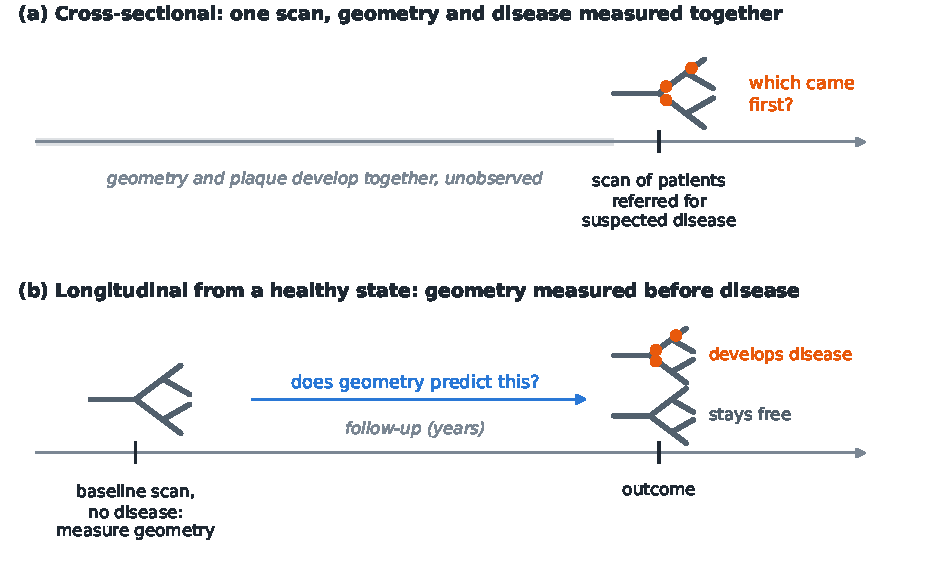
\includegraphics[width=0.9\textwidth]{rq_design.pdf}
  \caption{Only a study that measures geometry before disease can show that geometry predicts disease.
    (a) A cross-sectional study scans patients once, after disease may already be present, so it
    cannot tell whether the geometry preceded the plaque or changed with it
    \cite{cui2017bifurcation,groves2009tortuosity}.
    (b) A longitudinal study scans people while healthy and follows them forward; this is the
    design that is essentially missing \cite{zhang2024curvature}.}
  \label{fig:rq-design}
\end{figure}

\medskip
\noindent Whether the geometry of a healthy coronary tree carries information about who will go on to
develop plaque has therefore not been tested, and it is the question this thesis asks.

\printbibliography

\end{document}
